\section{Measures to maximise impact}

\subsection{Dissemination and exploitation of the results}

One of the most important parts of the project is the maximization of the impact of the products. This can be achieved by carrying out an exhaustive dissemination and exploitation of the results. Through a proper Dissemination Management Plan, the actions, needs and requirements for satisfactory results are defined. 

\textbf{Dissemination Management Plan}

The Dissemination Management Plan is designed in order to fulfil the dissemination and exploitation of the results of the project. The actions to perform are defined from the starting point of the project to the last stages after the project. It contains information about internal, stakeholders and external communication.

\begin{figure}[H]
	\centering
	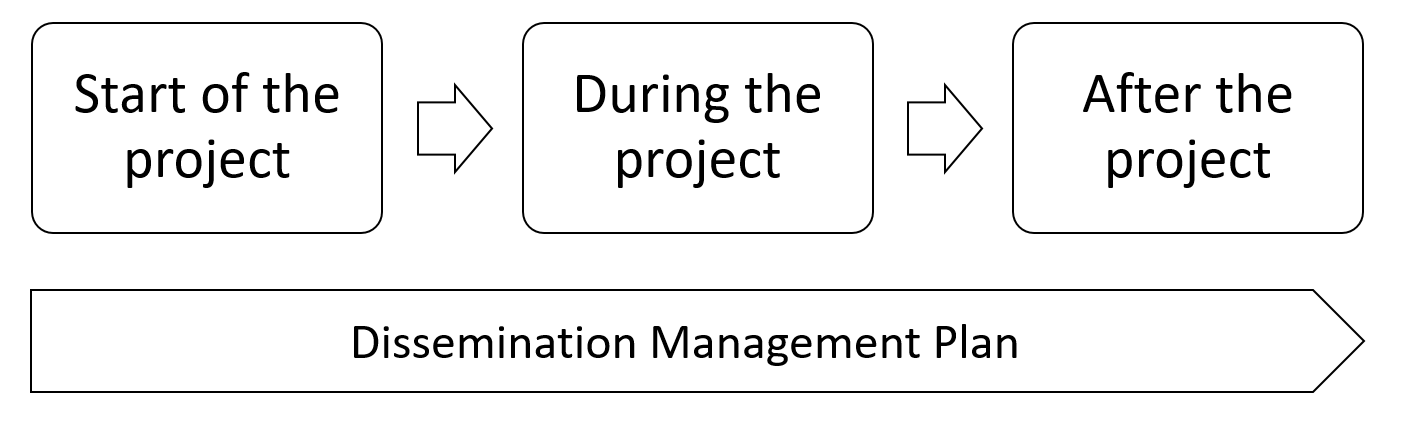
\includegraphics[width=\textwidth]{images/dissemination.png}
	\caption{Dissemination diagram} 
	\label{dissemination}
\end{figure}

Although internal communication is very important for the proper development of the project, we must not forget that external communication is also crucial in a project of this magnitude. Having a good dissemination plan involves explaining how the outcomes of the project will be shared with stakeholders, relevant institutions, organisations, and individuals. \\
In order to achieve the proposed objectives in terms of external communication, the process of dissemination will be focused  in two different ways depending on whether we want to reach the general public or aerospace sector.

\textbf{General public}

It is important to find an adequate channel to reach the less specialized public in the aerospace field. In order to achieve the maximum diffusion of the project in this sector,  the following resources will be used.

\begin{itemize}
	\item{\textbf{Social Networking.} Social networks are the best way to reach the widest possible audience. Posting regularly is also crucial to keep people interested in the project. Some of the platforms that will be used during the project development are: Twitter, Linkedin, Facebook, and Instagram. There will be at least one update a week in order to keep people informed of the progress of the project.}
	\item{\textbf{Website.} A project website is one of the most versatile dissemination tools and will help to reach people unfamiliar with social networks. It can contain information intended to different profiles. As in the previous case, it has to be kept updated.}
\end{itemize}

\textbf{Aerospace sector}

\begin{itemize}
	\item{\textbf{Trade shows.} Trade shows, fairs, and exhibitions are a great way to get in close contact with people from other regions and countries that we would ordinarily never be face to face with. They are also helpful in terms of finding new prospects, nurture current client relationships and stay up to date on the latest industry developments.}
	\item{\textbf{Conferences.} National and international conferences will help to share the achievements of the project with specialists in the field.}
	\item {\textbf{Journal Articles.} To promote project ideas and results in scientific research.}
\end{itemize}

\textbf{Information Management}

\begin{table}[H]
	\centering
	\begin{tabular}{p{7cm} p{7cm}}
		
		\toprule[2pt]
		
		\textbf{Question} &  \textbf{Description}\\
		
		\midrule [1.5pt]
		
		What types of data will the project generate/collect?  & This project will generate sensors data, ranging from pure images, to sensors data maps for analysing different aspects in each pixel.\vspace{0.2cm}\\
		
		\midrule
		
		What standards will be used?  & EU sensors manufacturing standrads will be used.\vspace{0.2cm}\\
		
		\midrule
		
		How will this data be exploited and/or shared/made accessible for verification and re-use? & Data will be post-process in order to extract valuable information. Will be shared along internet encrypted connection. Part of the data will be keep protected because is strategically sensible, hence involves key urban maps.\vspace{0.2cm}\\
		
		\midrule
		
		How will this data be curated and preserved? & It will be preserveted on a protected server.\vspace{0.2cm}\\
		
		\midrule
		
		How will the costs for data curation and preservation be covered? & The costs of data preservation will be covered by the clients payments, in this case, EU budget for the project.\vspace{0.2cm}\\	
		
		\bottomrule[2pt]
		
	\end{tabular}
	\caption{Information Management}
\end{table}

\textbf{Knowledge Management}

Knowledge management is the process of creating, sharing, using and managing the knowledge and information of an organisation. In the case of this project, the produced information has been classified into three groups that are explained below.

The first one consists of the public information of the project such as social media publications, the overall status of the project, open conferences, etc. The second will have the project status reports and deliverables and will be available to all the stakeholders. Finally, the third one, and the most restrictive, will be formed by confidential information, for instance, the technical methodologies and systems.

\begin{figure}[H]
	\centering
	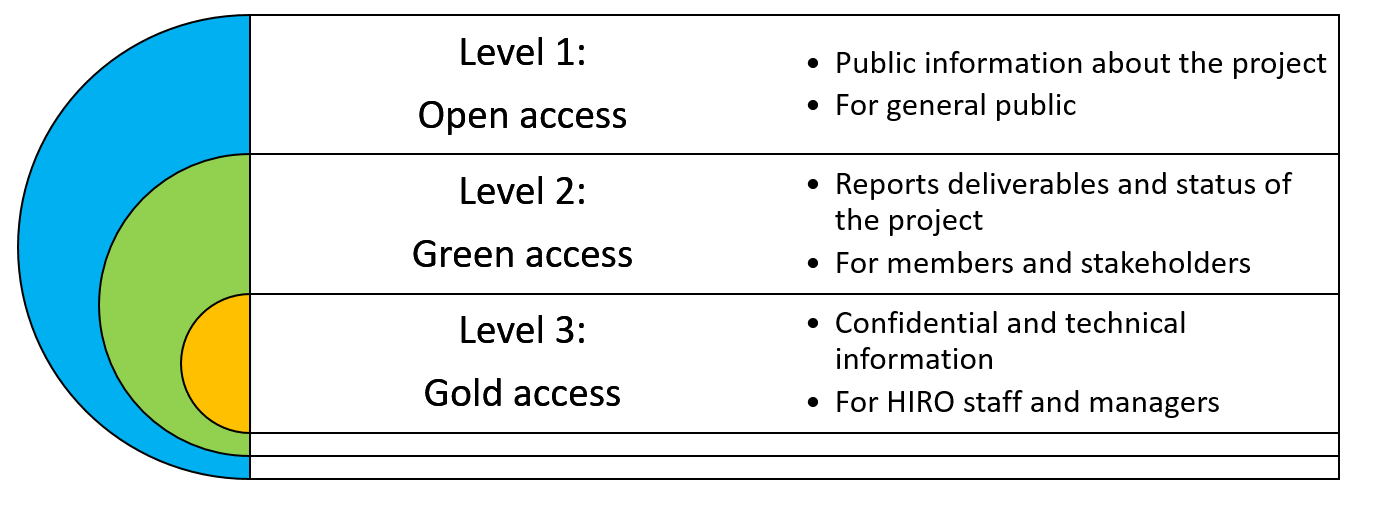
\includegraphics[width=\textwidth]{images/knowledgement.png}
	\caption{Levels of confidentiality} 
	\label{knowledge}
\end{figure}

All this information will be located in a private server and published in a website. Each group will have its own password to access to the Open, Green or Gold levels.

\subsection{Communication activities}

The following table shows the main communication actions in order to ensure a proper dissemination. It is also presented the medium, frequency, audience, owner, deliverable and format.

\begin{landscape}
	
	\begin{longtable}{| >{\raggedright\arraybackslash}p{2.8cm}  | >{\raggedright\arraybackslash}p{2.8cm} | >{\raggedright\arraybackslash}p{2cm} | >{\raggedright\arraybackslash}p{2cm} | >{\raggedright\arraybackslash}p{2cm} | >{\raggedright\arraybackslash}p{2.4cm} | >{\raggedright\arraybackslash}p{2.4cm} | >{\raggedright\arraybackslash}p{2.4cm} |  }
		
		\toprule [2pt]
		
		\textbf{Communication Type} & \textbf{Objective of Communication} & \textbf{Medium}  &\textbf{Frequency} &\textbf{Audience}& \textbf{Owner}& \textbf{Deliverable} &\textbf{Format} \\  
		
		\midrule [1.5pt]
		\endhead
		
		Social Networking& Share any updates on the project  & Facebook, Twitter, Instagram   &Weekly   &General Public     &  Marketing and Communication Manager &Online Posts   &Online\\  
		
		\hline
		
		Website& Contain varied information about the project  &   Website &Updated with any change   &  General Public   &  Marketing and Communication Manager & Online Posts  &Online\\  
		
		\hline
		
		Trade Shows&Face to face contact with potential customers as well as finding new prospects, nurture client relationships and stay up to date with latest developments   &  Onsite stands  & Scheduled  &  Potential Customers, Genera Public and Industry Professionals   &Marketing and Communication Manager   & None  &Face to Face\\  
		
		\hline
		
		Conferences& Sharing achievements with industry specialists  &  Conferences  &Scheduled   & Industry Professionals    & Project Manager  & Presentation  &Face to Face\\  
		
		\hline
		
		Journal Articles&Promoting project ideas, concepts and results in scientific and applied research communities and getting feedback from relevant stakeholders   &Digital and Written platforms    &  When Available &  Potential Customers, General Public and Industry Professionals   & Project Manager  & Journal Article  &Hard Copy\\  
		
		\bottomrule[2pt]
		
		\caption{Communication management plan matrix}
	\end{longtable}
	
	\vspace*{\fill}
		
\end{landscape}